\chapter{Nestor example 1}
%

% - Purpose & Problem description:
%     These first two parts give reader short details about the test case,
%     the physical phenomena involved and specify how the numerical solution will be validated
%
\section{Purpose}
%
First test example for Nestor
%
\section{Description of the problem}
%
This example is for testing dredging and dumping of the previously dredged material.

100 m$^3$ material will be dredged in the polygon named \texttt{201\_Abschnitt\_1\_2\_1000m**2}  defined in \texttt{\_DigPolys.dat} over a time period of 100 s.
The name must start with an integert number between 100 and 999. From position 4 is free text to help the user.
Only the number is the identifyer of the polygon. This Dredging area is located between 100,5 and 300,5 m of the flume with an area of 200 x 5 = 1000 m$^2$. In this part only
coarse material (dm=2mm) exists.
The dredging starts 50 s after the simulation start (2000.01.01-00:00:50) and ended 100 s later
(2000.01.01-00:02:30). This is defined in \texttt{\_DigActions.dat}.
The dredged material will create a final erosion of 0,1 m in the dredging area.
The dredging rate (calculeted by Nestor) is the dredging volume devided by the dredging time and the dredging area
$\frac{100 m^3/s}{100 s*1000 m^2}=0,001$ m/s

At the time when the dredging starts the dredged material will
be dumped in the polygon named \texttt{field 202\_Abschnitt\_6\_7\_1000m**2}, which is located between 700,5 and 900,5 m of the flume
with an area of 200 x 5 = 1000 m$^2$. The final sedimentation will be 0,1 m in the dumping field.
In this part originally only fine material is located (dm=0,1mm).
Due to a small dumping rate (preset to 0,0005 m/s), which is two times smaller than the dredging rate it takes 200 s to dump the material.

The sediment distribution will not be changed in the dredging area. In the
dumping area the mean grain size will be increased during the dumping of coarse material.
The final mean grain size is only 1,3 mm due to mixing processes of the Hirano layer model.
Without mixing processes, the active layer would completely consists of the coarse material and would have
a mean grain size of 2 mm as the sedimentation depth is as big as the active layer.

% - Physical parameters:
%     This part specifies the geometry, details all the physical parameters
%     used to describe both porous media (soil model in particularly) and
%     solute characteristics (dispersion/diffusion coefficients, soil <=> pollutant interactions...)
%
%
\subsection{Physical parameters}
%
The simulation has set up with three grain classes (d=0,1 / 0,2 / 2 mm), but only the fine and the coarse material
are used. The bottom is discretised with three layers. A constant active layer (10 cm), an underlying stratum (10 cm)
and a last layer up to the rigid bed (9.8m).

The Meyer-Peter Mueller transport formula is used but the MPM parameter is set to zero which avoids sediment transport.
All bottom changes come from the dredging and dumping processes.
% - Geometry and Mesh:
%     This part describes the mesh used in the computation
%
%
\subsection{Geometry and Mesh}
%
A 1000 m long flume with three widening parts has been chosen as test geometry (see figure \ref{ini}).
The width of the flume is 10 m and increases up to 30 m in the widening parts.
Two of the widening parts are 100 m long and the third is 200 m long.
The initial bottom has a continuous slope of 0,09 %.
The node area for every node is 1 m$^2$ in order to calculate dredging and dumping volumes very easily.

\begin{figure} [!h]
\centering
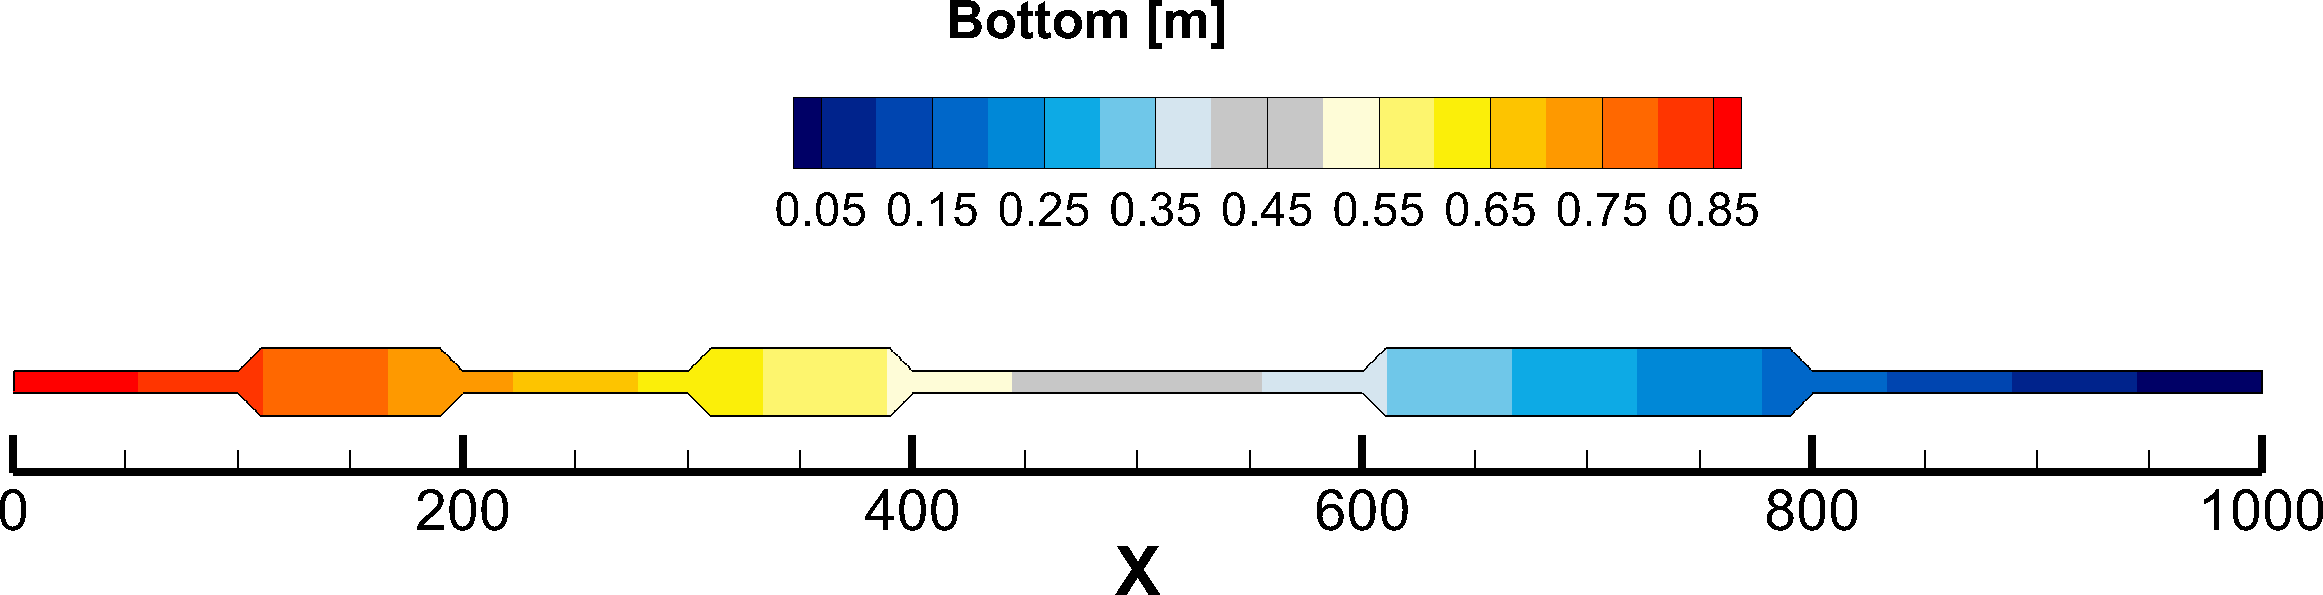
\includegraphics[scale=0.15]{../img/ini_bottom.png}
 \caption{Geometry of the test flume with three widening parts}\label{ini}
\end{figure}
The mesh consists of 18411 nodes and 34800 elements.

% - Initial and boundary conditions:
%     This part details both initial and boundary conditions used to simulate the case
%
%
\subsection{Initial and Boundary Conditions}
%
Steady state boundary conditions:
\begin{itemize}
\item{ Discharge at the inlet = 20 m$^3$/s}
\item Water depth at outlet = 1 m
\item Sedimentological equilibrium at the inlet (zF is constant, QS will be calculated)
\end{itemize}
Fully developed flow from a previous simulation is used as initial conditions.

With a time step of 1 s a simulation period of 250 s are computed.
% - Numerical parameters:
%     This part is used to specify the numerical parameters used
%     (adaptive time step, mass-lumping when necessary...)
%
%
\subsection{Numerical parameters}
%
% - Results:
%     We comment in this part the numerical results against the reference ones,
%     giving understanding keys and making assumptions when necessary.
%
%
\section{Results}
%
Figure \ref{result50} shows the evolution after 50 s (start of dredging and dumping),
after 100 s (end of dredging) and after 250 s (final simulation state and end of dumping process).

% Here is an example of how to include the graph generated by validateTELEMAC.py
% They should be in test_case/img
\begin{figure} [!h]
\centering
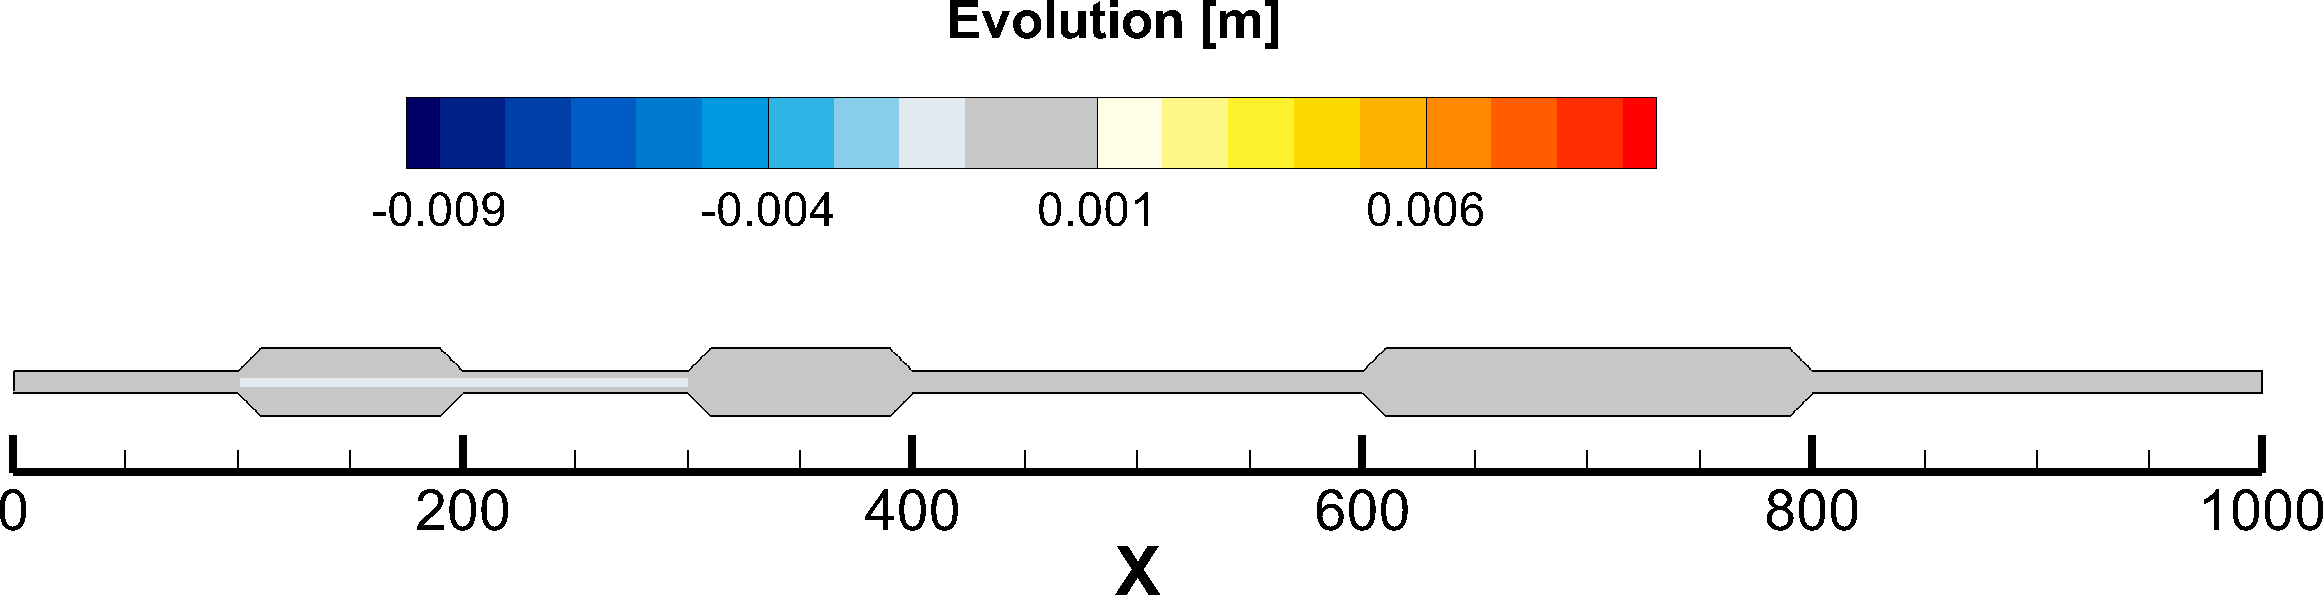
\includegraphics[scale=0.15]{../img/result50.png}
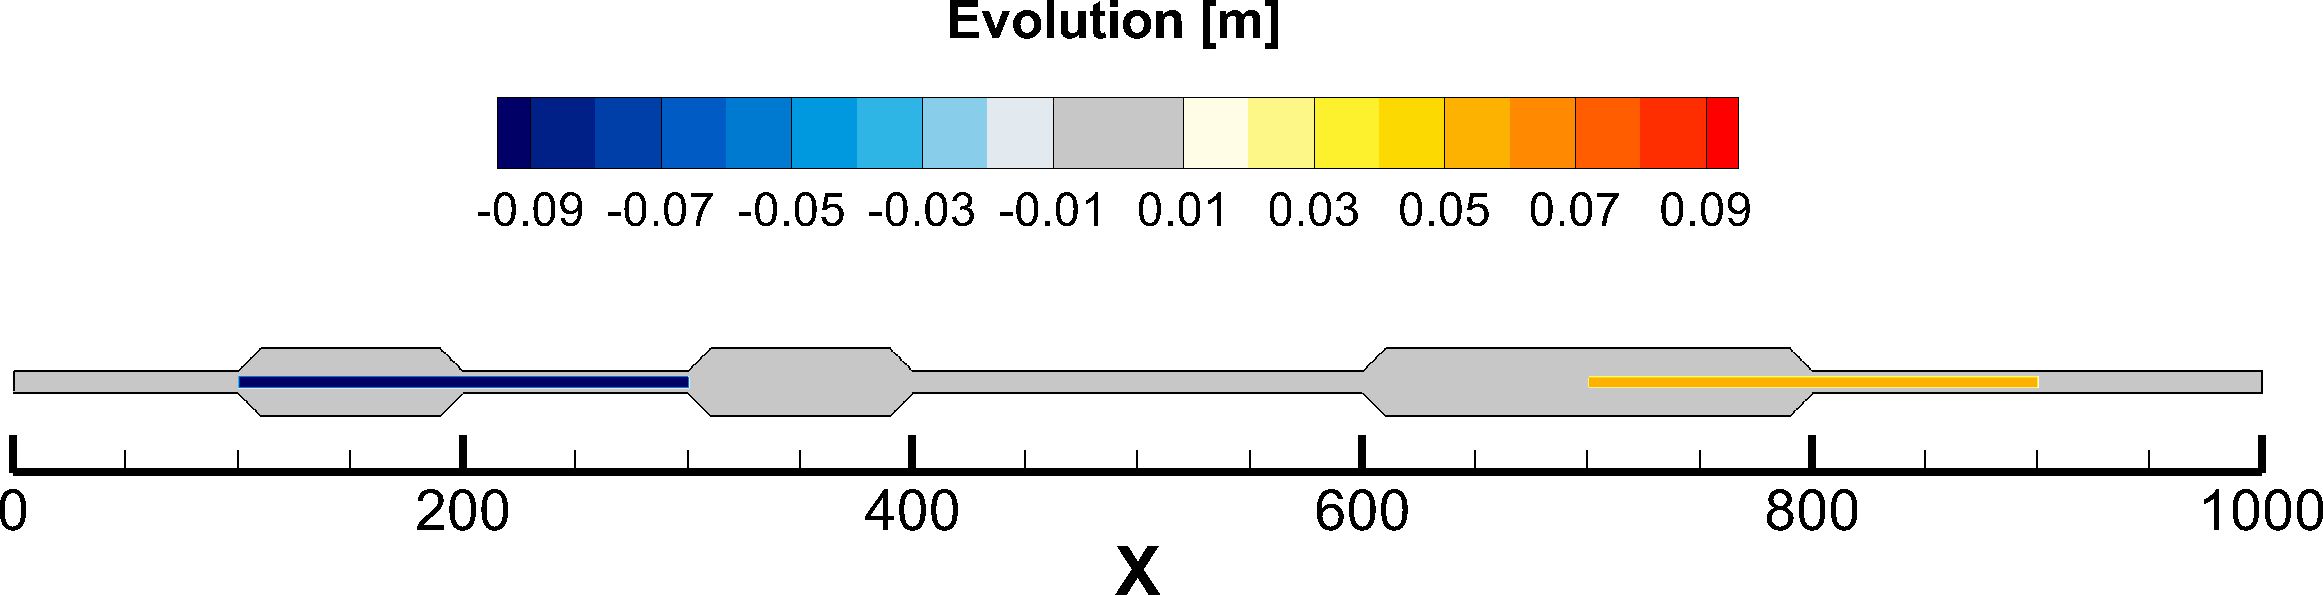
\includegraphics[scale=0.15]{../img/result150.png}
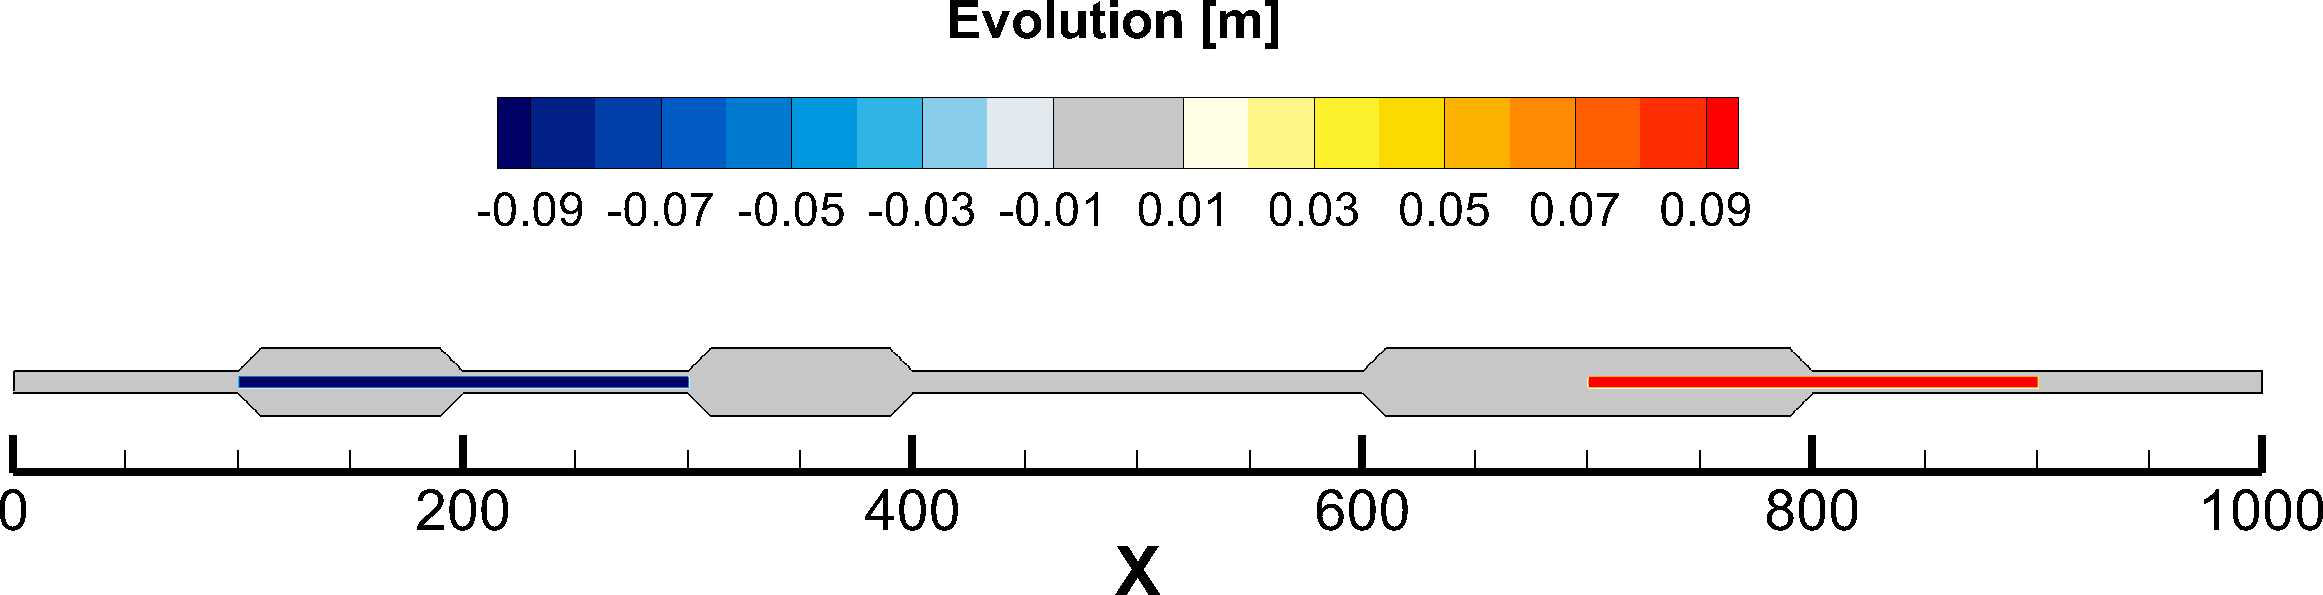
\includegraphics[scale=0.15]{../img/result250.png}
 \caption{Simulated evolution after 50, 100 and 250 s.}\label{result50}
\end{figure}


